\scanpage{76}
\mspage{75}

hand, \inserted{\handwritten{\uline{once one has chosen} \uline{a closure} $\overline{\mathbb{F}}_p$,}}\handwritten{\begin{tikzpicture}[baseline=0cm,x=1cm,y=1cm]\draw[thin] (0,-.4)--(0,.15)..controls (0,.22) and (.2,.21)..(.45,.21)--(4.5,.25)..controls (5.2,.18) and (5.4,.2)..(5.5,.55);\end{tikzpicture}} the gerbe $\handwritten{\underline{\pi}}_p(\underline{F}_p)$, thanks to the \deleted{its} obvious \unsure{\rlap{e}f|f}\unsure{\rlap{v}i|v|i|ï}bre functor ``fibre at $\handwritten{\bar{\underline{F}}}_p$ '' on the category of constructible $\underline{Q}_p$-sheaves on $\underline{F}_p$, is identified with the \deleted{category}\inserted{trivial gerbe defined\deleted{\unsure{and}} by .the} $\underline{Q}_p$-alg\unsure{e|e}braic envelope of the profinite group $\handwritten{\pi}_1(\underline{F}_p)=\handwritten{\bar{\underline{Z}}}\deleted{r}$, \deleted{which, as one readily observes, is the}

A constructible \inserted{$\underline{Q}_p$-}\handwritten{\begin{tikzpicture}[baseline=0cm,x=1cm,y=1cm]\draw[thin] (0,-.3)..controls (-.05,-.05) and (.55,.05)..(.7,.5);\end{tikzpicture}}sheaf on $\underline{F}_p$ is identified with a finite-dimensional vector space $E$ over $\underline{Q}_p$, equipped with an automorphism $F_E$ such that the \deleted{hom} action $n\handwritten{\mapsto}F_E^n$ of $\underline{Z}$ on $E$ extends by continuity to an action of \deleted{\unsure{$\hat{\underline{Z}}_r$|$\hat{\underline{Z}}r$}} $\handwritten{\hat{\underline{Z}}}$ \margin{\handwritten{$Z$}}. Identifying \inserted{\handwritten{(by a functor $j$, \uline{distinct} from the one in 5\unsure{,|.}2)}}\handwritten{\begin{tikzpicture}[baseline=0cm,x=1cm,y=1cm]\draw[gray,thin] (0,-.3)--(0,.15)--(6,.24)..controls (6.25,.25) and (6.4,.3)..(6.42,.48);\end{tikzpicture}} the category of these $(E,\unsure{\mathbb{E}_E|\deleted{E_E}|\rlap{F}E_E}F_E)$ with a\handwritten{\begin{tikzpicture}[baseline=0cm,x=1cm,y=1cm]\draw[gray,thin] (0,-.4)--(.28,.5);\end{tikzpicture}}full subcategory of\deleted{\unsure{s}} the category \deleted{of the} $\mathrm{Fcriso}(\underline{Q}_p)$ of pairs $(E,F_E)$, where $F_E$ is an \uline{arbitrary} automorphism, one sees that the band \deleted{of our}\inserted{$G\handwritten{'}$ of} $\handwritten{\underline{\pi}}_p(\underline{F}_p)$ of this category is identified with a quotient of the band $G$ of $\mathrm{Fcriso}(\underline{F}_p)$ determined above, and one sees at once that this quotient is of the form $G_u\mathrm{x}G_r^{\overset{\deleted{\unsure{2|a|x}}}{\handwritten{'}}}$, where $G_r'$ is \unsure{\rlap{h}th|th|h}\unsure{\rlap{e}e|e|e} quotient of $G_r$ (this amounts to saying that if one decomposes $F_E$ into the product of its unipotent component with its semi-simple component, then the condition that $F_E$ \unsure{\rlap{e}d|d}ef\unsure{\rlap{t}i|i}nes an action of $\handwritten{\hat{\underline{Z}}}$ depends only on the semi-simple component); precisely, $G'_r$ is the quotient group of $G_r$ defined by the subgroup of the character group $\handwritten{\bar{\underline{Q}}}_p^{\handwritten{*}}$ of $G_r$ consisting of the p\unsure{\rlap{é}-|é|-}\uline{adic} \uline{units} : this means in fac\unsure{\rlap{y}t|t} that $F_E$ defines an action of \deleted{$\unsure{F|G}_E$} $\handwritten{\hat{\underline{Z}}}$ (i.e. defines an F-isocrystal of slope zero) if and only if the eigenvalues\deleted{\unsure{s}} of $F_E$ are units, which indeed follows at once from the criterion given above for F-isocrystals of slope zero (or is verified directly in an immediate way; the reference to the result on the slope-zero gadgets should be justified by a grain of salt, for the inclusion \unsure{\rlap{y}u|u}sed here of constructible $\underline{Q}_p$-sheaves on $\underline{F}_p$ into\deleted{\unsure{d|to}} the F-iso\deleted{cr}crystals is not the one used \deleted{further \unsure{\rlap{y}u|u}p}\inserted{\handwritten{in 5.2}}, cf. below). One finds in thi\unsure{\rlap{i}s|s} fash\unsure{\rlap{s}i|i}on an extension structure on $G\handwritten{\unsure{\mathrel{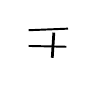
\begin{tikzpicture}[baseline=-.1cm,x=1cm,y=1cm]\draw[line width=.7pt] (0,.18)--(.5,.2);\draw[line width=.7pt] (0,-.02)--(.48,-.03);\draw[line width=1pt] (.32,.15)--(.3,-.17);\end{tikzpicture}}}}\operatorname{Lien}(\underline{G}(\underline{F}_p))$:
\[
0\handwritten{\longrightarrow}H\handwritten{\longrightarrow}G\handwritten{\longrightarrow}G'\handwritten{\mathrel{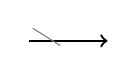
\begin{tikzpicture}[baseline=0cm,x=1cm,y=1cm]\draw[->,thick] (0,0)--(1,0);\draw[gray,thin] (.05,.16)--(.4,-.06);\end{tikzpicture}}}0\ ,
\]
where $H$ is the group of multiplicative type whose character group is the
